\documentclass[../main.tex]{subfiles}
\begin{document}
\chapter{Analisi del problema}

\section{Analisi traffico di rete}

Nell'era digitale il traffico di rete è aumentato notevolmente e con esso gli attacchi di tipo informatico, per questo motivo è necessario trovare soluzioni per analizzare questo grande quantitativo di pacchetti che attraversano i dispositivi di rete delle aziende di grosse dimensioni. Nel mondo informatico di oggi è molto importante poter determinare rapidamente e con precisione l'origine e la portata di un potenziale attacco su una rete al fine di poterlo contrastare in modo efficace.
Per fare ciò viene costruito un \textit{audit trail} di informazioni collezionate dal traffico di rete usando una combinazione di network flow e PCAP.

Un audit trail è un file che contiene una registrazione cronologica di attività relative alla sicurezza per consentire la ricostruzione e l'esame di eventi \cite{auditTrail}.

\subsection{Network Flow}
Un flow è una sequenza di pacchetti inviati da una sorgente ad una destinazione che hanno degli attributi in comune \cite{trafficflow}:
\begin{itemize}
				\item indirizzo IP sorgente
				\item indirizzo IP destinazione
				\item porta sorgente
				\item porta destinazione
				\item protocollo
\end{itemize}

Se i pacchetti che attraversano un dispositivo di rete hanno questi attributi in comune possono essere raggruppati in un flow.

\subsection{Packet Capture}
Per packet capture (PCAP) si intende la cattura di traffico internet che attraversa un dispositivo di rete. Un packet capture intercetta i singoli pacchetti e li archivia. Nei sistemi operativi Unix è utilizzata la libreria \textbf{libpcap} mentre nei sistemi Windows si fa utilizzo di \textbf{WinPcap} \cite{pcap}.

\subsection{NetFlow}
NetFlow è un protocollo di analisi di rete introdotto da Cisco che offre la possibilità di raccogliere informazioni dettagliate sul traffico mentre attraversa un'interfaccia. I dispositivi di rete che supportano NetFlow possono raccogliere statistiche sul traffico ed esportarle come record verso un NetFlow collector, un server che esegue l'analisi del traffico.

Cisco definisce un flow come una sequenza unidirezionale di pacchetti che condividono tutti i seguenti 7 valori \cite{netflowDef}.

\begin{itemize}
				\item interfaccia di ingresso
				\item indirizzo IP sorgente
				\item indirizzo IP destinazione
				\item protocollo IP
				\item porta sorgente TCP o UDP, 0 per altri protocolli
				\item IP Type of Service
\end{itemize}


\subsubsection{Componenti di NetFlow}
La figura 3.1 descrive un esempio di architettura dei network flow. 

\begin{figure}[H]
\centering
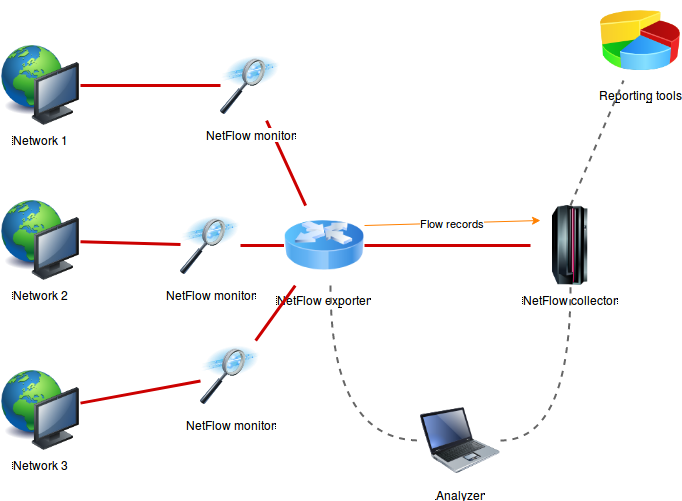
\includegraphics[scale=0.6]{netflowgraph.png}
\caption{Architettura NetFlow}
\end{figure}

\begin{verse}
\textbf{NetFlow monitor}
Un componente applicato a un'interfaccia che raccoglie informazioni sui flow. I NetFlow monitor sono costituiti da un record e una cache.
\end{verse}

\begin{verse}
\textbf{NetFlow exporter}
Aggrega i pacchetti in flows e ne esporta i record verso uno o più \textit{flow collectors}.
Quando dei pacchetti arrivano al NetFlow exporter, vengono ispezionati singolarmente per uno o più attributi che vengono utilizzati per determinare se il pachetto è univoco o è simile agli altri pacchetti. Se il pacchetto presenta attributi simili viene classificato nello stesso flow.


\begin{figure}[H]
\centering
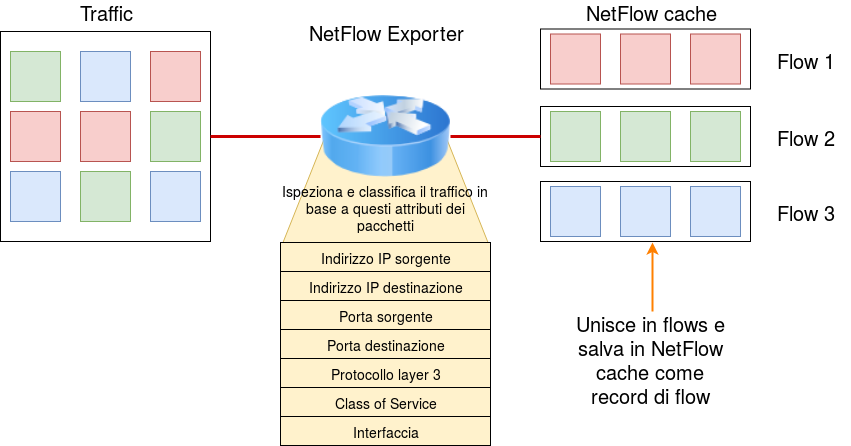
\includegraphics[scale=0.5]{netflowexporter.png}
\caption{NetFlow exporter}
\end{figure}

Dopo aver esaminato questi attributi, il NetFlow exporter li aggrega in record di flow e li salva in un database che può essere una cache NetFlow o un NetFlow collector.
\end{verse}

\begin{verse}
\textbf{NetFlow collector}
Responsabile della ricezione, conservazione e pre-elaborazione dei dati di un flow ricevuti da un \textit{flow exporter}. Solitamente è un software separato in esecuzione su un server di rete. I record NetFlow vengono esportati in un NetFlow collector tramite protocollo UDP.
\end{verse}

\begin{verse}
\textbf{Analysis application} 
Analizza i dati dei flows ricevuti nel contesto del rilevamento delle intrusioni o del profilo di traffico. Un esempio di Analysis application possono essere degli IDPS.
Di seguito un'immagine di SolarWinds NetFlow Traffic Analyzer, un esempio di analysis application.

\begin{figure}[H]
\centering
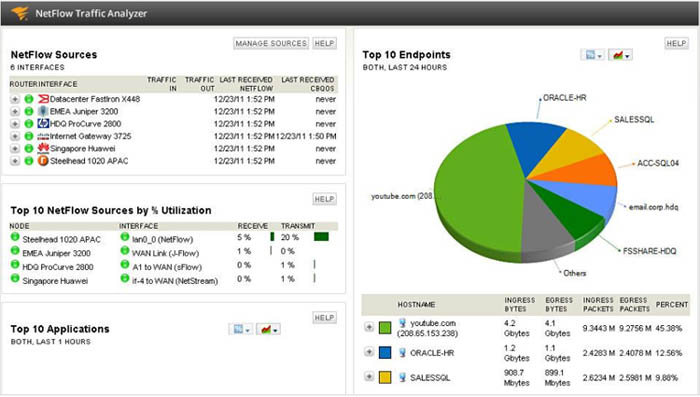
\includegraphics[scale=0.5]{netflowreport.jpg}
\caption{SolarWinds NetFlow Traffic Analyzer}
\end{figure}
\end{verse}

---- il nome della sezione va cambiato ---
\section{Strumenti software utilizzati}
---- riscrivere meglio ----
Verranno ora descritti i software utilizzati in questa tesi. I software utilizzati sono multipiattaforma, in questa tesi sono stati adoperati su sistema operativo basato su una distribuzione GNU/Linux.

\subsection{Audit Record Generation and Utilization System}
Argus (Audit Record Generation and Utilization System) è stato la prima implementazione del monitoraggio dei flow, è un progetto open source e multipiattaforma.
Quest'ultima particolarità lo rende molto interessante poichè supportando molti sistemi operativi, tra i quali Windows, MaxOSX, Linux, Solaris, FreeBSD, OpenBSD, IRIX e OpenWrt, può essere adoperato in quasi tutte le reti comprendendo la maggior parte degli host. La sua architettura è di tipo server/client. Il server recupera i pacchetti ricevuti da una o più interfacce di rete disponibili su una una macchina, argus assembla poi questi pacchetti in dati binari che rappresentano dei flow. Lo scopo dei client è di quello di leggere i dati dei flow. \newline

Argus viene utilizzato da molte università e aziende per registrare dei flow che vengono utilizzati sia nell'analisi immediata dell'utilizzo della rete, sia nell'analisi storica.

I file di Argus sono compressi con algoritmi che offrono un rapporto di compressione fino 10.000:1. La compressione di questi file è molto importante perchè sono file molto grandi e possono raggiungere dimensioni difficili da gestire. \newline


La seguente tabella descrive i campi dei flow che argus salva su file.
---- introdurre tabella ----

\begin{table}[h]
\begin{tabular}{|l|l|}
\hline
\textbf{campo} & \textbf{descrizione}                    \\ \hline
StartTime      & record start time                       \\ \hline
Dur            & record total duration                   \\ \hline
Proto          & transaction protocol                    \\ \hline
SrcAddr        & source IP address                       \\ \hline
Sport          & source port number                      \\ \hline
Dir            & direction of transaction                \\ \hline
DstAddr        & destination IP address                  \\ \hline
Dport          & destination port number                 \\ \hline
State          & transaction state                       \\ \hline
sTos           & source TOS byte value                   \\ \hline
dTos           & destination TOS byte value              \\ \hline
TotPkts        & total transaction packet count          \\ \hline
TotBytes       & total transaction bytes                 \\ \hline
SrcBytes       & src -\textgreater dst transaction bytes \\ \hline
srcUdata       & source user data buffer                 \\ \hline
dstUdata       & destination user data buffer            \\ \hline
Label          & metadata label                          \\ \hline
\end{tabular}
\end{table}

\subsection{nProbe}

Negli ambienti commerciali, NetFlow è probabilmente lo standard de facto per la gestione del traffico di rete. nProbe è un software in grado di reccogliere, analizzare ed esportare report sul traffico di rete utilizzando il formato standard Cisco NetFlow. È disponibile per la maggior parte dei sistemi operativi sul mercato. \newline

La tabella seguente descrive i campi dei flow che il software nProbe salva su file.

\begin{table}[H]
\begin{tabular}{|l|l|}
\hline
\multicolumn{1}{|c|}{\textbf{campo}} & \multicolumn{1}{c|}{\textbf{descrizione}}     \\ \hline
IPV4\_SRC\_ADDR                      & IPv4 source address                           \\ \hline
IPV4\_DST\_ADDR                      & IPv4 destination address                      \\ \hline
IPV4\_NEXT\_HOP                      & IPv4 next hop address                         \\ \hline
INPUT\_SNMP                          & input interface SNMP idx                      \\ \hline
OUTPUT\_SNMP                         & output interface SNMP idx                     \\ \hline
IN\_PKTS                             & incoming flow packets (src -\textgreater dst) \\ \hline
IN\_BYTES                            & incoming flow bytes (src -\textgreater dst)   \\ \hline
FIRST\_SWITCHED                      & SysUptime (msec) of the first flow pkt        \\ \hline
LAST\_SWITCHED                       & SysUptime (msec) of the last flow pkt         \\ \hline
L4\_SRC\_PORT                        & IPv4 source port                              \\ \hline
L4\_DST\_PORT                        & IPv4 destination port                         \\ \hline
TCP\_FLAGS                           & cumulative of all flow TCP flags              \\ \hline
PROTOCOL                             & IP protocol byte                              \\ \hline
SRC\_TOS                             & Type of service byte                          \\ \hline
SRC\_AS                              & source BGP AS                                 \\ \hline
DST\_AS                              & destination BGP AS                            \\ \hline
IPV4\_SRC\_MASK                      & IPv4 source subnet mask                       \\ \hline
IPV4\_DST\_MASK                      & IPv4 dest subnet mask                         \\ \hline
L7\_PROTO                            & layer 7 protocol (numeric)                    \\ \hline
BIFLOW\_DIRECTION                    & 1=initiator, 2=reverseInitiator               \\ \hline
FLOW\_START\_SEC                     & seconds (epoch) of the first flow packet      \\ \hline
FLOW\_END\_SEC                       & seconds (epoch) of the last flow packet       \\ \hline
OUT\_PKTS                            & outgoing flow packets (dst -\textgreater src) \\ \hline
OUT\_BYTES                           & outgoing flow bytes (dst -\textgreater src)   \\ \hline
FLOW\_ID                             & serial flow identifier                        \\ \hline
FLOW\_ACTIVE\_TIMEOUT                & activity timeout of flow cache entries        \\ \hline
FLOW\_INACTIVE\_TIMEOUT              & inactivity timeout of flow cache entries      \\ \hline
IN\_SRC\_MAC                         & source MAC address                            \\ \hline
OUT\_DST\_MAC                        & destination MAC address                       \\ \hline
\end{tabular}
\end{table}

---- argus vs nprobe ----

\section{Stratosphere IPS}
In questa tesi si è utilizzato Stratosphere IPS, un software open source disponibile per sistemi operativi Windows e distribuzioni GNU/Linux. In questa tesi si è fatto utilizzo esclusivo della versione per distribuzioni GNU/Linux.
Stratosphere Linux IPS (slips), al ---corrente----pubblicato come alpha, è un sistema di rilevazione e prevenzione delle intrusioni comportamentale che utilizza algoritmi di machine learning per rilevare comportamenti dannosi. 
L'obiettivo di Stratosphere IPS è quello di creare un Intrusion Prevention System che può rilevare e bloccare comportamenti malevoli all'interno di una rete.

---- introdurre nello stato dell'arte e descrivere qui in dettaglio il tipo ---
\begin{verse}
\textbf{Algoritmi di machine learning}
insieme di metodi di calcolo che utilizzano l'esperienza per migliorare le prestazioni o per effettuare delle previsioni accurate.
\end{verse}

---- riscrivere ----
\subsection{Architettura}
Slips si occupa della parte di rilevazione attraverso machine learning. Il traffico di rete viene letto da e salvato da Argus che rimane in ascolto su una porta. Slips legge poi i flows passati da standard input dal client di Argus. 
In questo modo è possibile analizzare il traffico del proprio computer o di qualsiasi altra rete su cui sia in esecuzione Argus.

\begin{figure}[H]
\centering
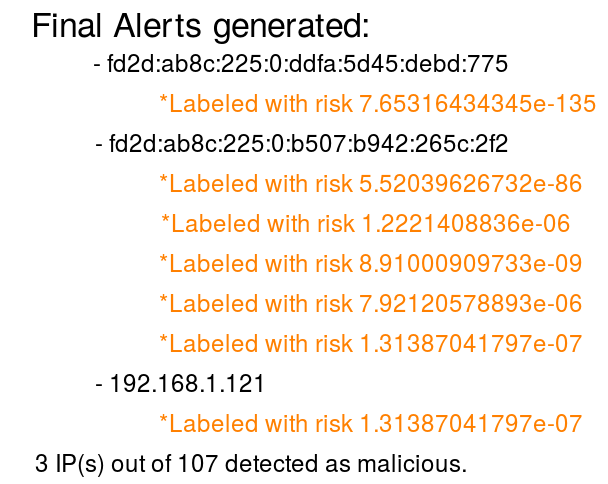
\includegraphics[scale=0.6]{slips.png}
\caption{Architettura Stratosphere}
\end{figure}

\subsection{Modelli comportamentali}
Slips fa utilizzo di modelli comportamentali creati da Stratosphere Testing Framework.

--- dire all'inizio della sezione la divisione del software in slips e stf ----
\begin{verse}
\textbf{Stratosphere Testing Framework}
è un framework di ricerca sulla sicurezza della rete per analizzare i modelli comportamentali delle connessioni di rete. Il suo obiettivo è aiutare i ricercatori a trovare nuovi comportamenti malware, etichettare tali comportamenti, creare i loro modelli di traffico e verificare gli algoritmi di rilevamento. Una volta creati e verificati i migliori modelli comportamentali di malware, questi verranno utilizzati da slips per il rilevamento. Stratosphere Testing Framework usa algoritmi di machine learning sui modelli comportamentali.
\end{verse}

Il nucleo di \textit{Stratosphere IPS} è composto dai modelli comportamentali di reti e algoritmi di rilevamento. I modelli comportamentali rappresentano ciò che una connessione specifica fa nella rete durante la sua vita. Il comportamento è costuito analizzando la sua periodicità, le dimensioni e la durata di ciascun flusso. Sulla base di queste caratteristiche a ciascun flusso viene assegnata una lettera e il gruppo di lettere caratterizza il comportamento della connessione.

--- dire i campi che influenzano i modelli ---

Prendiamo come esempio una connessione generata da una botnet che ha il seguente modello comportamentale
\begin{lstlisting}[language=bash]
88*y*y*i*H*H*H*y*0yy*H*H*H*y*y*y*y*H*h*y*h*h*H*H*h*H*y*y*y*H*
\end{lstlisting}

In questo caso ci dice che i flussi sono altamente periodici (lettere \textit{h}, \textit{i}), con qualche periodicità persa vicino all'inizio (lettere \textit{y}). I flussi hanno anche una grande dimensione con una durata media. I simboli tra le lettere sono correlati al tempo trascorso tra i flussi. In questo caso il simbolo '\textit{*}' significa che il flusso è separato da meno di un'ora.
Con l'utilizzo di questo tipo di modelli siamo in grado di generare le caratteristiche comportamentali di un gran numero di azioni dannose. L'immagine seguente mostra i criteri di assegnazione delle lettere per i modelli comportamentali \newline

--- introdurre l'immagine ----
\begin{figure}[H]
\centering
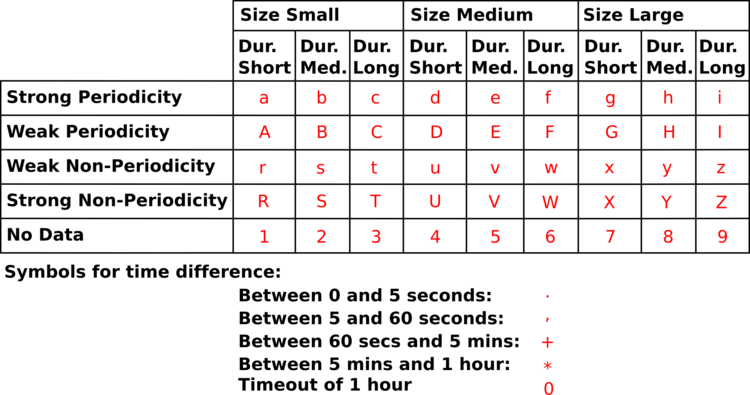
\includegraphics[scale=0.5]{modello-comportamentale.png}
				\caption{Tabella modelli comportamentali}
\end{figure}

\section{Problematiche dovute all'utilizzo di due diversi formati}
I file prodotti da nProbe e Argus, oltre ad avere formati diversi, hanno anche campi eterogenei. Stratosphere IPS si appoggia ad Argus per la cattura di file e di conseguenza può leggere file solo in formato binetflow. 
Se una azienda si appoggia a Cisco utilizzando nProbe non può quindi fare utilizzo di questo software, poichè non riesce a leggere file in formato differente.

Questa incompatibilità ha portato alla necessità di una conversione: i file prodotti da nProbe devono essere convertiti in file con formato usato da Argus. Questa conversione deve essere precisa ed efficiente.

\section{Presentazione del problema}
I file prodotti da nProbe hanno una struttura gerarchica fissa ben definita: ci sono 4 livelli di subdir, in cui il primo livello indica l'anno, il secondo il mese, il terzo il giorno e il quarto l'ora. All'interno dell'ultima subdir, quella delle ore, ci sono 60 file uno per ogni minuto della giornata.

--- introdurre l'immagine ----
\begin{figure}[H]
\centering
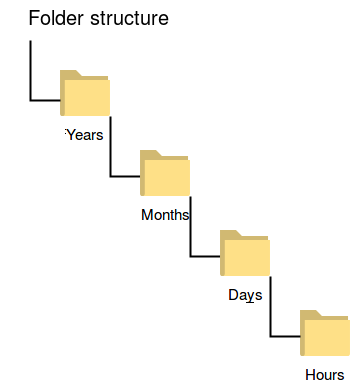
\includegraphics[scale=0.6]{folderstructure.png}
\caption{Folder Structure}
\end{figure}

\end{document}
